\chapter{Systemdesign} % (fold)
\label{sec:systemdesign}
Innerhalb dieses Abschnitts werden die konkret gewählten Technologien für die Entwicklung eines Systems beschrieben, das für Latentztests verwendet werden kann.
\section{Datenbankdesign} % (fold)
Für die Durchführung des Experiments wurden zwei Datenbanktypen verwendet, die nachfolgend mit ihrer spezifischen Konfiguration beschrieben werden.
\label{sec:datenbankdesign}
\subsection{Relationales Datenbankdesign} % (fold)
\label{sec:relationalesdatenbankdesign}

\begin{figure}[H]
	\centering
	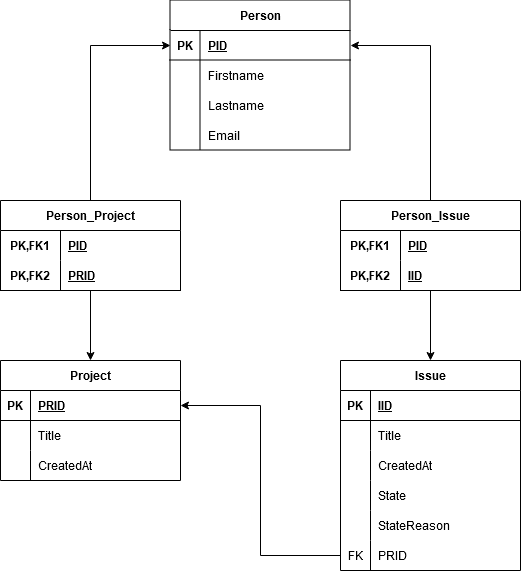
\includegraphics[scale=0.6]{Illustrations/table_diagram.png}
	\caption{Datenbankdiagramm}
\end{figure}
\newpage
\noindent
Für die Erstellung einer relationale Datenbank aus dem gegebenen Datenmodell (Abb. 4.1) wurde dieses wie in Abb. 5.1 zu sehen angepasst, um die Beziehung zwischen \texttt{Person} und \texttt{Project} sowie \texttt{Person} und \texttt{Issue} abzubilden. Somit ergeben sich für die relationale Datenbank fünf Tabellen, die in einer PostgreSQL- Datenbank realisiert werden. Dabei wird PostgreSQL verwendet, weil es ein leistungsfähiges, objekt-relationales Open-Source-Datenbanksystem bietet. Die Datenbank wurde mit den in Abbildung 5.2 bis 5.6 beispielhaft dargestellten Beispieldaten befüllt, wobei 500 000 \texttt{Person}- sowie \texttt{Project}- und \texttt{Issue}-Objekte in die Datenbank eingefügt wurden. Durch die Verwendung von Zwischentabellen, wie \texttt{Person\_Issue} und \texttt{Person\_Project}, enthält die relationale Datenbank 2,5 Mio. Tupel mit einem Speicherbedarf von 215 MB. 

\begin{figure}[H]
	\centering
	\begin{tabular}{|l | l | l | l |}
	\hline
	pid & firstname & lastname & email \\
	\hline
	1 & Cecilla & Beningfield & cbeningfield9@wp.com \\
	\hline
	\end{tabular}
	\caption{Tupel der Tabelle ‚Person‘}
\end{figure}
\begin{figure}[H]
	\centering
	\begin{tabular}{|l | l |}
	\hline
	pid & iid \\
	\hline
	1 & 4894 \\
	\hline
	\end{tabular}
	\caption{Tupel der Tabelle ‚Person\_Issue‘}
\end{figure}
\begin{figure}[H]
	\centering
	\begin{tabular}{|l | l | l | l | l | l|}
	\hline
	iid & title & createdat & state & statereason & prid \\
	\hline
	1 & Dabfeed & 2023-06-10 00:00:00 & Open & Assigned & 586 \\
	\hline
	\end{tabular}
	\caption{Tupel der Tabelle ‚Issue‘}
\end{figure}
\begin{figure}[H]
	\centering
	\begin{tabular}{|l | l |}
	\hline
	pid & prid \\
	\hline
	1 & 714 \\
	\hline
	\end{tabular}
	\caption{Tupel der Tabelle ‚Person\_Project‘}
\end{figure}
\begin{figure}[H]
	\centering
	\begin{tabular}{|l | l | l |}
	\hline
	prid & title & createdat \\
	\hline
	1 & Asoka & 2022-02-17 00:00:00 \\
	\hline
	\end{tabular}
	\caption{Tupel der Tabelle ‚Project‘}
\end{figure}
\newpage


% subsection relationalesdatenbankdesign (end)
\subsection{Graphdatenbankdesign} % (fold)
\label{sec:graphsdatenbankdesign}
Die Erstellung einer Graphdatenbank erfordert keine definierten Tabellen, weil sie die Daten schemafrei speichert. Die Kanten werden bei der Erstellung entsprechend den Objekten benannt, was ebenso auf die Beziehungen zwischen den Knoten zutrifft. Als Graphdatenbank wurde auf Neo4j als eine der am weitesten verbreiteten Graphdatenbanken zurückgegriffen, die eine hohe Benutzerfreundlichkeit bietet. Abbildung 5.7 bietet eine Demonstration einer Beziehung zwischen jeweils einem Knoten. Die Kanten sind als gerichtete Kanten abgebildet, wobei \texttt{Person} zwei ausgehende Kanten, \texttt{Project} zwei eingehende und \texttt{Issue}jeweils sowohl eine eingehende als auch eine ausgehende Kante aufweist. Wie in der relationalen Datenbank wurden auch in der Graphdatenbank 500 000 Knoten pro Objekt erstellt. Hierbei waren jedoch keine Zwischentabellen zur Darstellung von Beziehungen nötig, wodurch in der Datenbank 1,5 Mio. Knoten vorliegen, die durch 2,01 Mio. Kanten verbunden sind. Hieraus ergibt sich eine Gesamtgröße von 197 MB.

\begin{figure}[H]
	\centering
	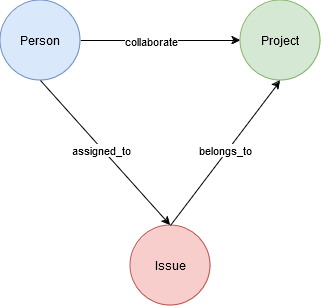
\includegraphics[scale=.8]{Illustrations/graph_diagram}
	\caption{Graphdiagramm}
\end{figure}
% subsection graphdatenbankdesign (end)

% section datenbankdesign (end)
\newpage
\section{Schnittstellendesign} % (fold)
\label{sec:schnittstellendesign}

\subsection{REST}
\label{sec:rest}
Bei REST wird für jedes Testszenario ein separater Endpunkt benötigt, wobei sechs Endpunkte mit unterschiedlicher Komplexität entworfen wurden.

\begin{itemize}
\item \colorbox{gray!20}{\textbf{HEAD api/resource}} wird verwendet, um einen Head-Request zur Bestimmung der Latenz der API durchzuführen..
\item Durch \colorbox{gray!20}{\textbf{GET api/issues?counter=x\&?joins=y}} kann die Menge der Ergebnistupel (x) und die Anzahl der auf der Datenbank durchgeführten Joins (y) bei der Anfrage bestimmt werden, wobei die in Abbildung 5.8 dargestellte Antwort erwartet wird.
\begin{figure}[H]
\begin{center}
\begin{BVerbatim}
   {
        "iid": 1,
        "title": "Pixope",
        "createdAt": "2024-07-23 00:00:00",
        "state": "Closed"
        "stateReason": "Cancelled"
    },
[...]
\end{BVerbatim}
\end{center}
\caption{‚GET api/issues?counter=x\&?joins=y‘-Response}
\end{figure}


\item \colorbox{gray!20}{\textbf{GET api/persons/:pid}}: Dieser Endpunkt ermöglicht das Abrufen einer bestimmten Person anhand ihrer ID, wobei die API ein JSON-Objekt zurückliefert, dass die \texttt{Person} mit den Attributen \texttt{Firstname, Lastname} und \texttt{E-Mail} beschreibt. (Abb. 5.9)
\begin{figure}[H]
\begin{center}
\begin{BVerbatim}
{
    "pid": 10,
    "firstname": "Cecilla",
    "lastname": "Beningfield",
    "email": "cbeningfield9@wp.com"
}
\end{BVerbatim}
\end{center}
\caption{‚GET api/persons/:pid‘-Response}
\end{figure}
\newpage
\item Mit dem Endpunkt  \colorbox{gray!20}{\textbf{GET api/persons}} können alle in der Datenbank gespeicherten Person- Objekte abgerufen werden, wobei die Antwort 5000  \texttt{Project}-Objekte im JSON-Format umfasst. (Abb. 5.10)
\begin{figure}[H]
\begin{center}
\begin{BVerbatim}
[
    {
        "pid": 1,
        "firstname": "Ruby",
        "lastname": "Burchatt",
        "email": "rburchatt0@msn.com"
    },
	[...]
    {
        "pid": 5000,
        "firstname": "Murdoch",
        "lastname": "Simonitto",
        "email": "msimonittorr@google.ca"
    }
]
\end{BVerbatim}
\end{center}
\caption{‚GET api/persons‘-Response}
\end{figure}

\item Der Endpunkt \colorbox{gray!20}{\textbf{GET api/persons/:pid/projects/issue}} erhöht die Komplexität, weil hier nicht nur auf ein einzelnes Objekt zugegriffen wird. Stattdessen erfordert die Abfrage zur Bearbeitung mehrere Objekte, die miteinander in Abhängigkeit stehen. Die Antwort umfasst alle  \texttt{Issue}-Objekte, die in  \texttt{Project}-Objekten vorhanden sind, in denen eine  \texttt{Person} mitwirkt. (Abb. 5.11)
\begin{figure}[H]
\begin{center}
\begin{BVerbatim}
[
   {
        "iid": 1,
        "title": "Pixope",
        "createdAt": "2024-07-23 00:00:00",
        "state": "Closed"
        "stateReason": "Cancelled"
    },
    {
        "iid": 2876,
        "title": "Zoomlounge",
        "createdAt": "2020-08-26 00:00:00",
        "state": "Open"
        "stateReason": "Bug"
    },
]
\end{BVerbatim}
\end{center}
\caption{‚GET api/persons/:pid/projects/issue‘-Response}
\end{figure}

\item Der Endpunkt \colorbox{gray!20}{\textbf{POST api/persons/:pid/projects/:prid/issues}} ermöglicht das Erstellen eines neuen Issue in der Datenbank, um nicht nur Abfragen, sondern auch das Hinzufügen von Daten zu testen. Im Body der Anfrage wird ein  \texttt{Issue}-Objekt im JSON-Format übergeben. (Abb. 5.12)
\newline
\begin{figure}[H]
\begin{center}
\begin{BVerbatim}
{
    "title":"test",
    "createdAt":"2023-02-21T00:00:00",
    "state":"Open",
    "stateReason":"Bug"
}
\end{BVerbatim}
\end{center}
\caption{‚POST api/persons/:pid/projects/:prid/issues‘-Body}
\end{figure}
\newpage
\noindent
Die Antwort enthält das erstellte \texttt{Issue}, das eine gültige  \texttt{ID} sowie Verknüpfungen zu dem zugehörigen  \texttt{Project} und der  \texttt{Person} umfassen. (Abb. 5.13)
\begin{figure}[H]
\begin{center}
\begin{BVerbatim}
{
    "iid": 5207,
    "title": "test",
    "createdAt": "2023-02-21T00:00:00",
    "state": "Open",
    "stateReason": "Bug",
    "project": {
        "prid": 12,
        "title": "Y-find",
        "createdAt": "2021-01-10T00:00:00"
    },
    "assignee"{
        "pid": 1,
        "firstname": "Ruby",
        "lastname": "Burchatt",
        "email": "rburchatt0@msn.com"
    },
}
\end{BVerbatim}
\end{center}
\caption{‚POST api/persons/:pid/projects/:prid/issues‘-Response}
\end{figure}
\end{itemize}

% section rest (end)
\newpage
\subsection{GraphQL}
Hinsichtlich der Art der Anfragen unterscheidet sich GraphQL stark von REST, denn es wird nur über den Endpunkt \colorbox{gray!20}{POST api/graphql}angesprochen, worüber sowohl Querys als auch Mutations abgedeckt werden. Die Anfragen werden im Body mithilfe der GraphQL-Query- Language definiert, die JSON ähnelt. Die in 5.2.1 definierten REST-Endpunkte wurden in GraphQL nachgebildet, sodass sie dieselbe Antwort liefern. Für einen HEAD-Request bietet GraphQL nativ jedoch keine Lösung, weshalb in GraphQL APIs der HEAD-Request identisch wie in den REST-APIs implementiert wurde. Der parametrisierte Endpunkt aus der REST-API wurde in GraphQL entsprechend der Darstellung in Abb. 5.14 umgesetzt, wobei bei \texttt{Counter} Werte zwischen 0 und 1,5 Mio sowie bei  \texttt{Joins} Werte zwischen 0 und 3 möglich sind.

\begin{figure}[H]
\begin{center}
\begin{BVerbatim}
query{
    issuesCount(counter: 10, joins: 1){
	iid
	title 
	createdAt 
	state 
	stateReason
    }
}
\end{BVerbatim}
\end{center}
\caption{GraphQ-Query GET api/issues?counter=x\&?joins=y}
\end{figure}
\noindent
Die in Abbildung 5.15 dargestellte Query ist dem REST-Endpunk \colorbox{gray!20}{GET api/persons/:pid} äquivalent, wobei ebenfalls eine ID übergeben wird. Allerdings können die in der Antwort enthaltenen Felder explizit gewählt werden. In diesem Beispiel wurden \texttt{PID},  \texttt{Firstname},  \texttt{Lastname} sowie die  \texttt{E-Mail} genutzt, um dieselbe Antwort wie beim REST-Endpunkt zu erhalten.
\begin{figure}[H]
\begin{center}
\begin{BVerbatim}
query{
    person(id : 10){
	pid
	firstname
	lastname
	email
    }
}
\end{BVerbatim}
\end{center}
\caption{GraphQL-Query-Äquivalent zu GET api/persons/:pid}
\end{figure}
\noindent
Der REST-Endpunkt \colorbox{gray!20}{GET api/persons} wird von der GraphQL-Query in Abbildung 5.16 repräsentiert, wobei dieselben Felder wie in der vorherigen Abfrage selektiert werden. Jedoch wird hierbei die Query \colorbox{gray!20}{persons} angesprochen, wodurch alle  \texttt{Person} Objekte der Datenbank abgerufen werden.
\begin{figure}[H]
\begin{center}
\begin{BVerbatim}
query {
    persons {
        pid
        firstname
        lastname
        email
    }
}
\end{BVerbatim}
\end{center}
\caption{GraphQL-Query-Äquivalent zu GET api/persons}
\end{figure}
\noindent
Abbildung 5.17 zeigt die GraphQL-Query, die dem REST-Endpunkt \colorbox{gray!20}{GET api/persons/} \colorbox{gray!20}{:pid/projects/issue} entspricht. Hierbei werden die im Schema definierten Querys geschachtelt, um eine Abfrage zu erhalten, die die Abhängigkeiten zwischen den Objekten repräsentiert.
\begin{figure}[H]
\begin{center}
\begin{BVerbatim}
query{
    person(id : 10){
        projects{
	    issues{
		iid
		title
		createdAt
		state
		stateReason
	    }
        }
    }
}
\end{BVerbatim}
\end{center}
\caption{GraphQL-Query-Äquivalent zu GET api/persons/:pid/projects/issue}
\end{figure}
\newpage
\noindent
Um den REST-Endpunkt \colorbox{gray!20}{POST api/persons/:pid/projects/:prid/issues} nachzubilden wurde die in Abb. 5.18 dargestellte Mutation entwickelt. Hierbei wird ein Input-Objekt definiert, das die zur Erstellung des Issue benötigten Attribute beinhaltet. Danach kann selektiert werden, welche Felder in der Antwort enthalten sind.
\begin{figure}[H]
\begin{center}
\begin{BVerbatim}
mutation{
    createIssue(input:{
	title : „Bug in Login“
	createdAt : „2024-12-03T12:30:00
	state : „Open“
	stateReason : „Error in Login“
	prid: 80
	pid: 10
	}){
	iid
	title
	state
	stateReason
	createdAt
	project{
	   prid
	   title
	   createdAt
	}
	assignee{
	   pid
	   firstname
	   lastname
	   email
	}
    }
}
\end{BVerbatim}
\end{center}
\caption{GraphQL-Query-Äquivalent zu POST api/persons/:pid/projects/:prid/issues}
\end{figure}

\label{sec:graphql}
% section graphql (end)

% section schnittstellendesign (end)
\newpage
\section{Testumgebung} % (fold)
\label{sec:testumgebung}
Zur Ermittlung der Latenzzeiten wurden API-Abfragen durchgeführt, wobei die Antwortzeiten in Millisekunden protokolliert wurden. Dafür wurde eine Testumgebung mit zwei unterschiedlichen Endgeräten benötigt, um die Last auf mehrere Geräte zu verteilen. Die APIs liefen auf einem Server in Frankfurt, der mit vier Kernen, 24 GB Arbeitsspeicher, einer 1 Gbit-Internetverbindung und Ubuntu 22.04 als Betriebssystem ausgestattet ist.
\newline
Die Abfragen erfolgten von einem PC mit acht Kernen, 32 GB Arbeitsspeicher, einer 50 Mbit- Internetverbindung und Windows 10 als Betriebssystem, wobei die durchschnittliche Latenz (Ping) zwischen Server und PC 24 ms betrug. Weil ein Ping jedoch nur auf ISO-Schicht 3 agierte, wurde vor jedem Testdurchlauf mithilfe von HEAD-Requests, die in Kapitel 5.2.1 beschrieben wurden, eine Latenz zwischen den Endgeräten ermittelt, die alle ISO-Schichten durchlief. Um Schwankungen bei der Netzwerkauslastung und der Systembelastung zu minimieren, wurden pro Testszenario und API jeweils hundert Anfragen ausgeführt. Insgesamt ergibt dies bei vier APIs und 25 Testszenarien eine Datengrundlage von 10 000 Latenzzeiten.


% section testumgebung (end)


% chapter Systemdesign (end)